\section{Polimorfismo de subtipos}
  \label{sec:oop:principios:clases_abstractas}

  La \textbf{serialización} es el proceso de convertir un objeto en un formato que pueda ser
  almacenado o transmitido y reconstruido posteriormente en el mismo o en un objeto similar.
  La serialización es un proceso muy útil para guardar el estado de un objeto en un archivo o
  transmitirlo a través de una red.

  Supongamos que queremos guardar nuestras cartas en archivos de distintos formatos: XML, JSON y
  YAML.
  Los formatos que queremos son los siguientes:

  \begin{xml}
    <!-- XML -->
    <MonsterCard>
      <name>White-eyes Blue Dragon</name>
      <text>Legendary dragon of destruction</text>
      <attack>3000</attack>
    </MonsterCard>
  \end{xml}

  \begin{json}
    // JSON
    {
      "name": "White-eyes Blue Dragon",
      "text": "Legendary dragon of destruction",
      "attack": 3000,
      "type": "MonsterCard"
    }
  \end{json}

  \begin{yaml}
    # YAML
    !!MonsterCard
    name: White-eyes Blue Dragon
    text: Legendary dragon of destruction
    attack: 3000
  \end{yaml}

  Con esto podemos hacer el proceso de serialización de la siguiente manera:

  \begin{kotlin}
    open class Card(name: String, text: String, attack: Int) {
      ...
      open fun toXml(): String {
        return """
          |<Card>
          |  <name>$name</name>
          |  <text>$text</text>
          |  <attack>$attack</attack>
          |</Card>
        """.trimMargin()
      }
      open fun toJson(): String {
        return """
          |{
          |  "name": "$name",
          |  "text": "$text",
          |  "attack": $attack
          |  "type": "Card"
          |}
        """.trimMargin()
      }
      open fun toYaml(): String {
        return """
          |!!Card
          |name: $name
          |text: $text
          |attack: $attack
        """.trimMargin()
      }
    }
  \end{kotlin}

  Y para las cartas de monstruo:

  \begin{kotlin}
    class MonsterCard(name: String, text: String, attack: Int) : Card(name, text, attack) {
      ...
      override fun toXml(): String {
        return """
          |<MonsterCard>
          |  <name>$name</name>
          |  <text>$text</text>
          |  <attack>$attack</attack>
          |</MonsterCard>
        """.trimMargin()
      }
      override fun toJson(): String {
        return """
          |{
          |  "name": "$name",
          |  "text": "$text",
          |  "attack": $attack
          |  "type": "MonsterCard"
          |}
        """.trimMargin()
      }
      override fun toYaml(): String {
        return """
          |!!MonsterCard
          |name: $name
          |text: $text
          |attack: $attack
        """.trimMargin()
      }
    }
  \end{kotlin}

  ¿Pero qué finalidad tiene definir las funciones \texttt{toXml()}, \texttt{toJson()} y 
  \texttt{toYaml()} en la clase \texttt{Card} si las vamos a sobreescribir en la clase que hereda
  de ella?
  Como veran, tenemos un problema.

  La idea sería poder definir una función en la clase carta sin tener que implementarla.
  Esto podemos lograrlo con \textbf{clases abstractas}.

  \begin{defaultbox}[Clase abstracta]
    Una clase abstracta\index{Clase abstracta} es una clase incompleta que no puede ser instanciada.

    Una función abstracta\index{Función abstracta} es una función que no tiene implementación.
    Para que una clase abstracta tenga sentido, debe tener al menos una función abstracta.
  \end{defaultbox}

  En \textit{Kotlin} las clases abstractas se definen con la palabra clave \texttt{abstract} y deben
  comenzar con la palabra clave \texttt{Abstract}.\footnote{
    Esto último es para hacer más fácil distinguir entre clases abstractas y clases concretas.
  }
  Comencemos por cambiar el nombre de la clase \texttt{Card} a \texttt{AbstractCard}, para esto 
  podemos darle click derecho al nombre de la clase y seleccionar la opción \texttt{Refactor ->
  Rename} como en la \cref{fig:oop:principios:clases_abstractas:rename}, esto cambiará el nombre de
  la clase en todos los archivos donde se use además de cambiar el nombre del archivo.

  \begin{figure}[ht!]
    \centering
    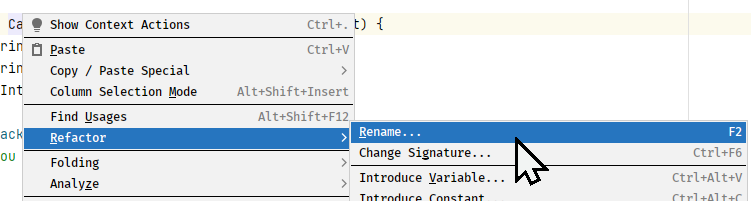
\includegraphics[width=0.8\textwidth]{img/oop/principios/clases_abstractas/idea64_rename.png}
    \caption{Renombrando la clase \texttt{Card} a \texttt{AbstractCard}.}
    \label{fig:oop:principios:clases_abstractas:rename}
  \end{figure}

  Ahora, agregamos la palabra clave \texttt{abstract} antes de la palabra clave \texttt{class} y
  cambiamos los métodos \texttt{toXml()}, \texttt{toJson()} y \texttt{toYaml()} a funciones
  abstractas:

  \begin{kotlin}
    abstract class AbstractCard(name: String, text: String, attack: Int) {
      ...
      abstract fun toXml(): String
      abstract fun toJson(): String
      abstract fun toYaml(): String
    }
  \end{kotlin}

  \begin{important}
    Las funciones abstractas deben ser implementadas en las clases que hereden de la clase
    abstracta.
  \end{important}

  ¿Qué sucede si ahora además quiero poder guardar las cartas en un archivo?
  Podríamos definir métodos para guardar las cartas en archivos de distintos formatos:

  \begin{kotlin}
    abstract class AbstractCard(name: String, text: String, attack: Int) {
      ...
      abstract fun toXmlFile(fileName: String)
      abstract fun toJsonFile(fileName: String)
      abstract fun toYamlFile(fileName: String)
    }
  \end{kotlin}

  Pero (para variar) tenemos un problema.
  Cada vez que queramos agregar un nuevo formato, tendremos que agregar una nueva función a la
  clase abstracta y luego implementarla en cada clase que herede de ella.
  Esto es un problema porque si tenemos muchas clases que hereden de la clase abstracta, tendremos
  que modificarlas todas cada vez que se agregue un nuevo formato.

  \begin{defaultbox}[Open-closed principle]
    \index{Open-closed principle}
    Las clases deben estar abiertas para extensión pero cerradas para modificación.
  \end{defaultbox}

  Una solución es delegar la responsabilidad de guardar las cartas en archivos a una clase que se 
  encargue de eso, aprovechando la propiedad de composición y polimorfísmo.

  \begin{defaultbox}[Polimorfísmo de subtipos]
    \index{Polimorfísmo de subtipos}
    El polimorfismo de subtipos es la propiedad de un objeto de tipo \(A\) de verse y ser usado como
    un objeto de tipo \(B\) siempre y cuando \(A\) sea un subtipo de \(B\).
  \end{defaultbox}

  En términos prácticos, esto significa que podemos crear una función \(f(B)\) y pasarle un objeto
  de tipo \(A\) siempre y cuando \(A\) sea un subtipo de \(B\).

  Pero antes de continuar ordenemos nuestro programa.
  Como notarán, a medida que avanzamos en el desarrollo del programa, la cantidad de archivos que
  tenemos va creciendo de forma acelerada.
  Esto es un problema porque si queremos modificar una clase, tenemos que ir a buscarla en todos
  los archivos.
  Una solución es agrupar las clases con características similares en paquetes.

  \begin{figure}[ht!]
    \centering
    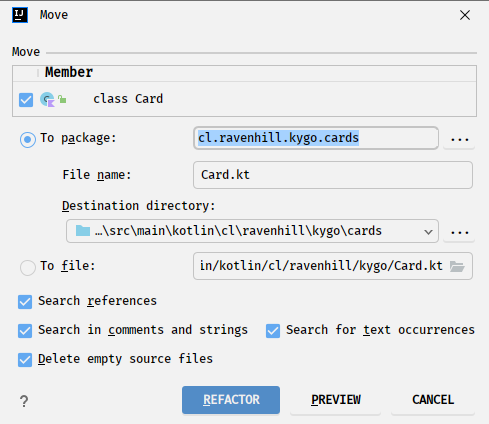
\includegraphics[width=0.5\textwidth]{img/oop/principios/clases_abstractas/idea64_move.png}
    \caption{Moviendo las clases \texttt{AbstractCard} y \texttt{MonsterCard} al paquete \texttt{cards}.}
    \label{fig:oop:principios:clases_abstractas:move}
  \end{figure}

  Hagamos un paquete \texttt{cards} haciendo click derecho en el paquete 
  \url{cl.ravenhill.kygo} y arrastremos los archivos \texttt{AbstractCard.kt} y
  \texttt{MonsterCard.kt} dentro de él, esto desplegará una ventana como la de la 
  \cref{fig:oop:principios:clases_abstractas:move} donde deberemos comprobar los cambios que se
  realizarán y luego darle click al botón \textit{Refactor}.
  Luego hagamos un paquete \texttt{serialization} en el paquete \url{cl.ravenhill.kygo}.

  Luego, creemos la clase \texttt{AbstractCardSerializer} en el paquete \texttt{serialization}, 
  recordando agregar la palabra clave \texttt{abstract} antes de la palabra clave \texttt{class}:

  \begin{kotlin}
    package cl.ravenhill.kygo.serializer

    import cl.ravenhill.kygo.cards.AbstractCard
    import java.io.File


    abstract class AbstractCardSerializer {
      fun toFile(card: AbstractCard, filename: String) {
        val file = File(filename)
        file.writeText(serialize(card))
      }

      abstract fun serialize(card: AbstractCard): String
    }
  \end{kotlin}

  Aquí tenemos algo nuevo: la clase \texttt{File} y el método \texttt{File::writeText(String)}.
  La clase \texttt{File} es una clase que representa un archivo en el sistema de archivos, y el
  método \texttt{File::writeText(String)} es un método que recibe un string y lo escribe en el
  archivo.

  Ahora podemos definir clases que hereden de \texttt{AbstractCardSerializer} para cada formato:

  \begin{kotlin}
    class XmlCardSerializer(card: AbstractCard) : AbstractCardSerializer() {
      private val card = card

      override fun serialize(): String {
        return """
          |<Card>
          |  <name>${card.name}</name>
          |  <text>${card.text}</text>
          |  <attack>${card.attack}</attack>
          |</Card>
        """.trimMargin()
      }
    }
  \end{kotlin}



  Y por último, podemos modificar la clase \texttt{AbstractCard} para que use la clase
  \texttt{AbstractCardSerializer}:

  \begin{kotlin}
    class AbstractCard(
      name: String, text: String, attack: Int, 
      serializer: AbstractCardSerializer) {
      ...
      var serializer = serializer

      fun toFile(filename: String) {
        serializer.toFile(this, filename)
      }

      fun serialize(): String {
        return serializer.serialize(this)
      }
    }
  \end{kotlin}

  Aquí nos topamos nuevamente con nuestro amigo \texttt{this}.
  En \textit{Kotlin} existen dos pseudo-variables que nos permiten referenciar a un objeto: 
  \texttt{this} y \texttt{super}.
  ¿Cuál es la diferencia entre ellas?
  Fácil, \texttt{this} hace referencia al objeto que recibe el mensaje, mientras que \texttt{super}
  hace referencia al objeto que recibe el mensaje.

  \begin{center}
    ¿Qué?
  \end{center}

  \begin{defaultbox}[\texttt{this} y \texttt{super}]
    \index{this}\index{super}
    Tanto \texttt{this} como \texttt{super} son pseudo-variables que hacen referencia al objeto que
    recibe un mensaje.

    Lo que hace distintos a \texttt{this} y \texttt{super} es el \textit{method-lookup}.
    En el caso de \texttt{this}, el \textit{method-looup} comienza en la clase del objeto que 
    recibe el mensaje, mientras que en el caso de \texttt{super}, el \textit{method-lookup} comienza 
    en la superclase del objeto que recibe el mensaje.
  \end{defaultbox}

  Ahora, nuestra clase \texttt{MonsterCard} debiera quedar así:

  \begin{kotlin}
    class MonsterCard(
      name: String,
      text: String,
      attack: Int,
      serializer: AbstractCardSerializer
    ) : AbstractCard(name, text, attack, serializer) {
      override fun attack(player: Player) {
        player.takeDamage(this.attack)
      }
    }
  \end{kotlin}

  ¿Lo ven venir?
  Tenemos un pequeño problema: estamos usando una clase abstracta como tipo.
  Este problema es un poco más complejo de ver, pero es importante entenderlo.
  Al declarar el tipo de la variable \texttt{serializer} como \texttt{AbstractCardSerializer},
  estamos diciendo que la variable es de un tipo que definimos como algo incompleto.
  ¿Existe una manera de representar tipos que agrupen a todos los tipos que hereden de una clase
  abstracta y que no sean abstractos?

  \begin{defaultbox}[Interfaces]
    Una interfaz es un contrato entre un cliente y un proveedor.
    Un proveedor declara las propiedades que tienen todos los objetos que representa y un cliente
    puede crear cualquier objeto que cumpla con el contrato de la interfaz.
  \end{defaultbox}

  \begin{important}
    Las interfaces son una forma de tener polimorfísmo de subtipos sin tener que usar herencia de 
    clases (porque una interfaz no es una clase).  
  \end{important}
  
  Las clases abstractas e interfaces son similares, pero tienen una diferencia importante.
  Como ya sabemos, una clase puede extender de solo una superclase, pero como una interfaz no es una
  clase, sino que un contrato, una clase puede implementar muchas interfaces siempre y cuando no
  rompa con el contrato de ninguna de ellas.
  
  En \textit{Kotlin} las interfaces se definen con la palabra clave \texttt{interface} en vez de
  \texttt{class}.

  Podemos crear una interfaz \texttt{CardSerializer} haciendo click derecho en el paquete
  \url{serializer} y seleccionando \textit{New} \texttt{->} \textit{Kotlin File/Class}.
  Luego, en la ventana que se despliega, seleccionamos \textit{Interface} y le damos un nombre a la
  interfaz, en este caso \texttt{CardSerializer}.
  Eso nos creará el siguiente archivo:

  \begin{kotlin}
    package cl.ravenhill.kygo.serializer

    interface CardSerializer {
    }
  \end{kotlin}

  Y ahora agregamos los métodos \texttt{serialize(AbstractCard): String} y 
  \texttt{toFile(AbstractCard, String)} a la interfaz:

  \begin{kotlin}
    interface CardSerializer {
      fun serialize(card: AbstractCard): String
      fun toFile(card: AbstractCard, filename: String)
    }
  \end{kotlin}

  Ahora, podemos modificar la clase \texttt{AbstractCardSerializer} para que implemente la interfaz
  \texttt{CardSerializer}, esto lo hacemos de la misma forma que heredamos de una clase, con la
  diferencia de que (al no ser clases) las interfaces no tienen constructor:

  \begin{kotlin}
    abstract class AbstractCardSerializer: CardSerializer {
      override fun toFile(card: AbstractCard, filename: String) {
        val file = File(filename)
        file.writeText(serialize(card))
      }

      abstract override fun serialize(card: AbstractCard): String
    }
  \end{kotlin}

  Y ahora podemos modificar la clase \texttt{AbstractCard} para que use la interfaz \texttt{CardSerializer}:

  \begin{kotlin}
    abstract class AbstractCard(
      name: String, text: String, attack: Int,
      serializer: CardSerializer
    ) {...}
  \end{kotlin}

  Como siempre, terminamos con:

  \begin{powershell}
    git add .
    git commit -m "FEAT Adds card serializers"
  \end{powershell}

  \begin{exercise}
    Cree una interfaz \texttt{Card} para no usar la clase \texttt{AbstractCard} como tipo.
  \end{exercise}
    
  \begin{exercise}
    Implemente las clases \texttt{JsonSerializer} y \texttt{YamlSerializer} que extiendan de
    \texttt{AbstractCardSerializer} y que implementen el método \texttt{serialize}.
  \end{exercise}